\chapter{\oracle: \EN{.SYM-files}\RU{.SYM-файлы}}
\index{\oracle}

\RU{Когда процесс в \oracle терпит серьезную ошибку (crash), он записывает массу информации в лог-файлы,
включая состояние стека, вроде:}
\EN{When \oracle process experiencing some kind of crash, it writes a lot of information into log files,
including stack trace, like:}

\begin{lstlisting}
----- Call Stack Trace -----
calling              call     entry                argument values in hex      
location             type     point                (? means dubious value)     
-------------------- -------- -------------------- ----------------------------
_kqvrow()                     00000000             
_opifch2()+2729      CALLptr  00000000             23D4B914 E47F264 1F19AE2
                                                   EB1C8A8 1
_kpoal8()+2832       CALLrel  _opifch2()           89 5 EB1CC74
_opiodr()+1248       CALLreg  00000000             5E 1C EB1F0A0
_ttcpip()+1051       CALLreg  00000000             5E 1C EB1F0A0 0
_opitsk()+1404       CALL???  00000000             C96C040 5E EB1F0A0 0 EB1ED30
                                                   EB1F1CC 53E52E 0 EB1F1F8
_opiino()+980        CALLrel  _opitsk()            0 0
_opiodr()+1248       CALLreg  00000000             3C 4 EB1FBF4
_opidrv()+1201       CALLrel  _opiodr()            3C 4 EB1FBF4 0
_sou2o()+55          CALLrel  _opidrv()            3C 4 EB1FBF4
_opimai_real()+124   CALLrel  _sou2o()             EB1FC04 3C 4 EB1FBF4
_opimai()+125        CALLrel  _opimai_real()       2 EB1FC2C
_OracleThreadStart@  CALLrel  _opimai()            2 EB1FF6C 7C88A7F4 EB1FC34 0
4()+830                                            EB1FD04
77E6481C             CALLreg  00000000             E41FF9C 0 0 E41FF9C 0 EB1FFC4
00000000             CALL???  00000000             
\end{lstlisting}

\RU{Но конечно, для этого исполняемые файлы \oracle должны содержать некоторую отладочную информацию,
либо map-файлы с инфомрацией о символах или что-то в этом роде.}
\EN{But of course, \oracle executables must have some kind of debug information or map files with symbol
information included or something like that.}

\RU{\oracle для Windows NT содержит информацию о символах в файлах с расширением .SYM, но его формат закрыт.}
\EN{Windows NT \oracle have symbol information in files with .SYM extension, but the format is proprietary.}
\EN{(Plain text files are good, but needs additional parsing, hence offer slower access.)}
\RU{(Простые текстовые файлы это хорошо, но они требуют дополнительной обработки (парсинга), и из-за этого доступ
к ним медленнее.)}

\RU{Посмотрим, сможем ли мы разобрать его формат}\EN{Let's see if we can understand its format}.
\RU{Я выбрал самый короткий файл \TT{orawtc8.sym}, поставляемый с файлом \TT{orawtc8.dll} в Oracle 8.1.7}
\EN{I chose shortest \TT{orawtc8.sym} file, coming with \TT{orawtc8.dll} file in Oracle 8.1.7}
\footnote{\RU{Я выбрал древнюю версию \oracle сознательно, из-за более короткого размера его модулей}\EN{I chose 
ancient \oracle version intentionally due to smaller size of its modules}}.

\clearpage
\RU{Вот я открываю этот файл в}\EN{Here is the file opened in} Hiew:

\begin{figure}[H]
\centering
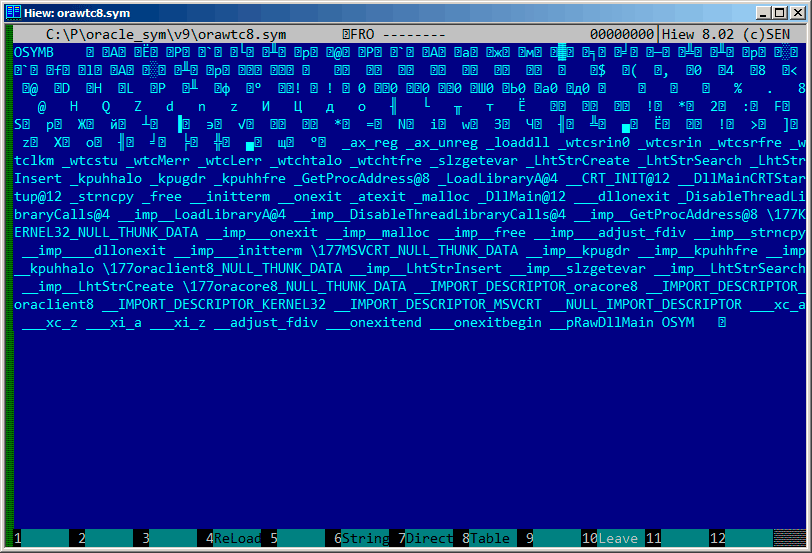
\includegraphics[scale=\FigScale]{ff/Oracle_SYM/whole1.png}
\caption{\RU{Весь файл в Hiew}\EN{The whole file in Hiew}}
\label{fig:oracle_SYM_whole1}
\end{figure}

\RU{Сравнивая этот файл с другими .SYM-файлами, мы можем быстро заметить что \TT{OSYM} всегда является
заголовком (и концом), так что это наверное сигнатура файла.}
\EN{By comparing the file with other .SYM files, we can quickly see that \TT{OSYM} is always header (and footer),
so this is maybe file signature.}

\RU{Мы также видим что в общем-то, формат файла это: OSYM + какие-то бинарные данные + 
текстовые строки разделенные нулем + OSYM.}
\EN{We also see that basically, file format is: OSYM + some binary data + zero delimited text strings + OSYM.}
\RU{Строки это, очевидно, имена ф-ций и глобальных переменных}\EN{Strings are, obviously, function and global 
variable names}.

\clearpage
\RU{Я отметил сигнатуры OSYM и строки здесь}\EN{I marked OSYM signatures and strings here}: 

\begin{figure}[H]
\centering
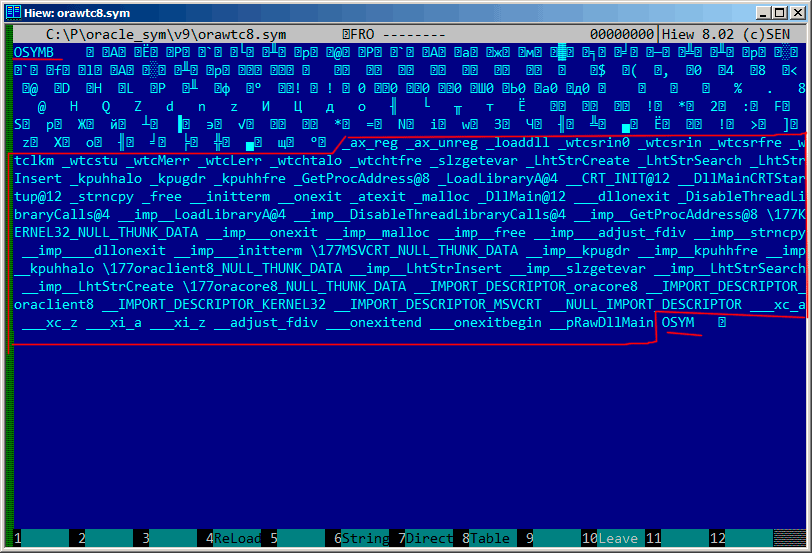
\includegraphics[scale=\FigScale]{ff/Oracle_SYM/whole2.png}
\caption{\RU{Сигнатура OSYM и текстовые строки}\EN{OSYM signature and text strings}}
\label{fig:oracle_SYM_whole2}
\end{figure}

\RU{Посмотрим}\EN{Well, let's see}. 
\RU{В Hiew я отметил весь блок со строками (исключая оконечивающую сигнатуру OSYM) и сохранил его в отдельный
файл.}
\EN{In Hiew, I marked the whole strings block (except trailing OSYM signatures) and put it into separate file.}
\RU{Затем я запустил UNIX-утилиты \IT{strings} и \IT{wc} для подсчета строк здесь:}
\EN{Then I run UNIX \IT{strings} and \IT{wc} utilities to count strings in there:}

\begin{lstlisting}
strings strings_block | wc -l
66
\end{lstlisting}

\RU{Так что здесь 66 текстовых строк}\EN{So there are 66 text strings}.
\RU{Запомните это число}\EN{Please note that number}.

\RU{Можно сказать, что в общем, как правило, количество \IT{чего-либо} часто сохраняется в бинарном
файле отдельно.}
\EN{We can say, in general, as a rule, number of \IT{anything} is often stored separately in binary files.}
\RU{Это действительно так, мы можем найти значение 66 (0x42) в самом начале файла, прямо после сигнатуры OSYM:}
\EN{It's indeed so, we can find 66 value (0x42) at the file begin, right after OSYM signature:}

\lstinputlisting{ff/Oracle_SYM/dump1.txt}

\RU{Конечно, 0x42 здесь это не байт, но скорее всего, 32-битное значение, запакованное как little-endian,
поэтому мы видим 0x42 и затем как минимум 3 байта.}
\EN{Of course, 0x42 here is not a byte, but most likely a 32-bit value, packed as little-endian, hence we see
0x42 and then at least 3 zero bytes.}

\RU{Почему я думаю что оно 32-битное}\EN{Why I think it's 32-bit}?
\RU{Потому что файлы с символами в \oracle могут быть очень большими}\EN{Because, \oracle symbol 
files may be pretty big}.
\RU{oracle.sym для главного исполняемого файла oracle.exe (версия 10.2.0.4) содержит \TT{0x3A38E} (238478) 
символов.}
\EN{The oracle.sym for the main oracle.exe (version 10.2.0.4) executable contain \TT{0x3A38E} (238478) symbols.}
\RU{16-битного значения тут недостаточно}\EN{16-bit value isn't enough here}.

\RU{Я проверил другие .SYM-файлы как этот и это подтвердило мою догадку: значение после 32-битной сигнатуры OSYM
всегда отражает количество текстовых строк в файле.}
\EN{I checked other .SYM files like this and it proves my guess: the value after 32-bit OSYM signature is always
reflects number of text strings in the file.}

\RU{Это общая особенность почти всех бинарных файлов: заголовок с сигнатурой плюс некоторая дополнительная
информация о файле.}
\EN{It's a general feature of almost all binary files: header with signature plus some other information 
about file.}

\RU{Рассмотрим бинарный блок поближе}\EN{Now let's investigate closer what this binary block is}.
\RU{Снова используя Hiew, я сохранил блок начиная с адреса 8 (т.е., после 32-битного значения,
отражающего количество) до блока со строками, в отдельный файл.}
\EN{Using Hiew again, I put the block starting at address 8 (i.e., after 32-bit \IT{count} value) 
till strings block into separate binary file.}

\clearpage
\RU{Посмотрим этот блок в}\EN{Let's see the binary block in} Hiew:

\begin{figure}[H]
\centering
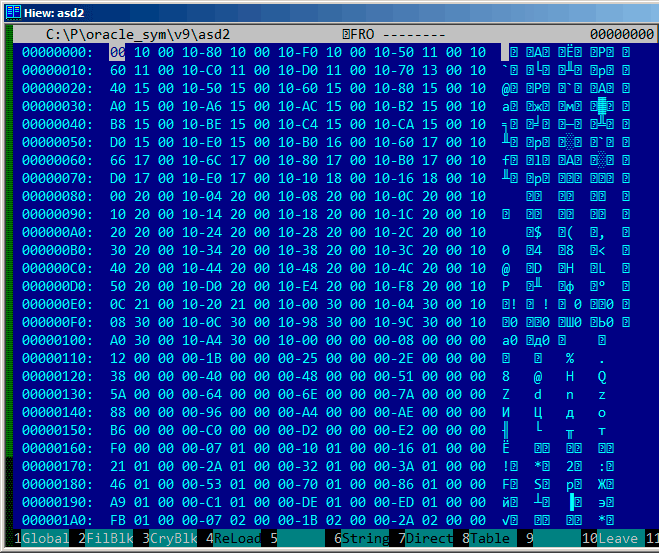
\includegraphics[scale=\FigScale]{ff/Oracle_SYM/binary1.png}
\caption{\RU{Бинарный блок}\EN{Binary block}}
\label{fig:oracle_SYM_binary1}
\end{figure}

\RU{Тут явно есть какая-то структура}\EN{There is some clear pattern in it}. 

\clearpage
\RU{Я добавил красные линии, чтобы разделить блок}\EN{I added red lines to divide the block}: 

\begin{figure}[H]
\centering
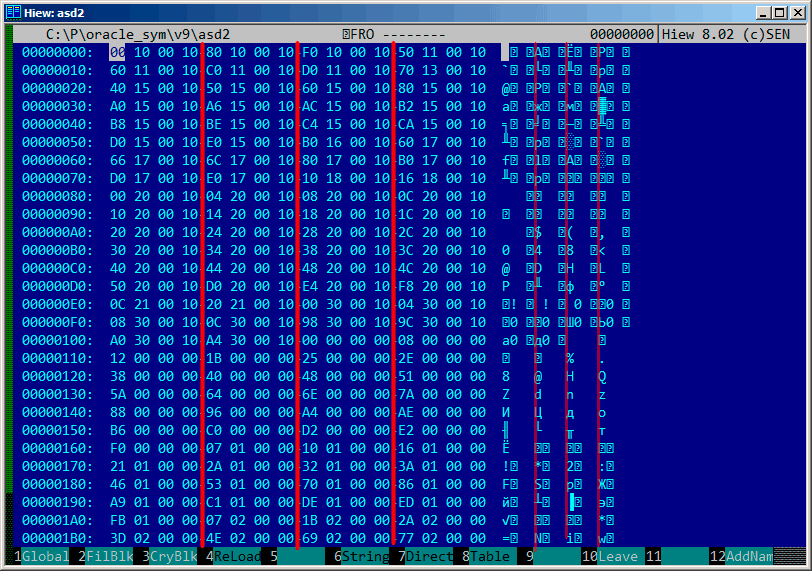
\includegraphics[scale=\FigScale]{ff/Oracle_SYM/binary2.png}
\caption{\RU{Структура бинарного блока}\EN{Binary block patterns}}
\label{fig:oracle_SYM_binary2}
\end{figure}

\RU{Hiew, как и многие другие шестнадцатеричные редакторы, показывает 16 байт на строку.}
\EN{Hiew, like almost any other hexadecimal editor, shows 16 bytes per line.}
\RU{Так что структура явно видна: здесь 4 32-битных значения на строку}\EN{So the pattern is clearly visible: 
there are 4 32-bit values per line}.

\RU{Эта структура видна визуально потому что некоторые значения здесь (вплоть до адреса \TT{0x104}) 
всегда в виде \TT{0x1000xxxx}, так что начинаются с байт 0x10 и 0.}
\EN{The pattern is visually visible because some values here (till address \TT{0x104}) 
are always in \TT{0x1000xxxx} form, 
so started by 0x10 and 0 bytes.}
\RU{Другие значения (начинающиеся на \TT{0x108}) всегда в виде \TT{0x0000xxxx}, так что начинаются с двух
нулевых байт.}
\EN{Other values (starting at \TT{0x108}) are in \TT{0x0000xxxx} form, so always started by two zero bytes.}

\RU{Посмотрим на этот блок как на массив 32-битных значений}\EN{Let's dump the block as 32-bit values array}:

\lstinputlisting[caption=\RU{первый столбец это адрес}\EN{first column is address}]{ff/Oracle_SYM/dump2.txt}

\RU{Здесь 132 значения, а это 66*2}\EN{There are 132 values, that's 66*2}.
\RU{Может быть здесь 2 32-битных значения на каждый символ, а может быть здесь два массива}\EN{Probably, 
there are two 32-bit values for each symbol, but maybe there are two arrays}? 
\RU{Посмотрим}\EN{Let's see}.

\RU{Значения, начинающиеся с}\EN{Values started with} \TT{0x1000} \RU{могут быть адресами}\EN{may be addresses}.
\RU{В конце концов, этот .SYM-файл для DLL, а базовый адрес для DLL в win32 это \TT{0x10000000}, и сам код
обычно начинается по адресу \TT{0x10001000}.}
\EN{This is .SYM file for DLL after all, and, default base address of
win32 DLLs is \TT{0x10000000}, and the code is usually started at \TT{0x10001000}.}

\RU{Когда я открываю файл orawtc8.dll в IDA, базовый адрес другой, но тем не менее, первая ф-ция это:}
\EN{When I open orawtc8.dll file in IDA, base address is different, but nevertheless, the first function is:}

\begin{lstlisting}
.text:60351000 sub_60351000    proc near
.text:60351000
.text:60351000 arg_0           = dword ptr  8
.text:60351000 arg_4           = dword ptr  0Ch
.text:60351000 arg_8           = dword ptr  10h
.text:60351000
.text:60351000                 push    ebp
.text:60351001                 mov     ebp, esp
.text:60351003                 mov     eax, dword_60353014
.text:60351008                 cmp     eax, 0FFFFFFFFh
.text:6035100B                 jnz     short loc_6035104F
.text:6035100D                 mov     ecx, hModule
.text:60351013                 xor     eax, eax
.text:60351015                 cmp     ecx, 0FFFFFFFFh
.text:60351018                 mov     dword_60353014, eax
.text:6035101D                 jnz     short loc_60351031
.text:6035101F                 call    sub_603510F0
.text:60351024                 mov     ecx, eax
.text:60351026                 mov     eax, dword_60353014
.text:6035102B                 mov     hModule, ecx
.text:60351031
.text:60351031 loc_60351031:                           ; CODE XREF: sub_60351000+1D
.text:60351031                 test    ecx, ecx
.text:60351033                 jbe     short loc_6035104F
.text:60351035                 push    offset ProcName ; "ax_reg"
.text:6035103A                 push    ecx             ; hModule
.text:6035103B                 call    ds:GetProcAddress
...
\end{lstlisting}

\RU{Ух ты}\EN{Wow}, ``ax\_reg'' \RU{звучит знакомо}\EN{string sounds familiar}. 
\RU{Действительно, это самая первая строка в блоке строк!}
\EN{It's indeed the first string in the strings block!}
\RU{Так что имя этой ф-ции, похоже}\EN{So the name of this function it seems} ``ax\_reg''.

\RU{Вторая ф-ция}\EN{The second function is}:

\begin{lstlisting}
.text:60351080 sub_60351080    proc near
.text:60351080
.text:60351080 arg_0           = dword ptr  8
.text:60351080 arg_4           = dword ptr  0Ch
.text:60351080
.text:60351080                 push    ebp
.text:60351081                 mov     ebp, esp
.text:60351083                 mov     eax, dword_60353018
.text:60351088                 cmp     eax, 0FFFFFFFFh
.text:6035108B                 jnz     short loc_603510CF
.text:6035108D                 mov     ecx, hModule
.text:60351093                 xor     eax, eax
.text:60351095                 cmp     ecx, 0FFFFFFFFh
.text:60351098                 mov     dword_60353018, eax
.text:6035109D                 jnz     short loc_603510B1
.text:6035109F                 call    sub_603510F0
.text:603510A4                 mov     ecx, eax
.text:603510A6                 mov     eax, dword_60353018
.text:603510AB                 mov     hModule, ecx
.text:603510B1
.text:603510B1 loc_603510B1:                           ; CODE XREF: sub_60351080+1D
.text:603510B1                 test    ecx, ecx
.text:603510B3                 jbe     short loc_603510CF
.text:603510B5                 push    offset aAx_unreg ; "ax_unreg"
.text:603510BA                 push    ecx             ; hModule
.text:603510BB                 call    ds:GetProcAddress
...
\end{lstlisting}

\RU{Строка ``ax\_unreg'' также это вторая строка в строке блок!}
\EN{``ax\_unreg'' string is also the second string in strings block!}
\RU{Адрес начала второй ф-ции это \TT{0x60351080}, а второе значение в бинарном блоке это \TT{10001080}.}
\EN{Starting address of the second function is \TT{0x60351080}, and the second value in the binary 
block is \TT{10001080}.}
\RU{Так что это адрес, но для DLL с базовым адресом по умолчанию}\EN{So this is address, 
but for the DLL with default base address}.

\RU{Я могу быстро проверить и убедиться что первые 66 значений в массиве (т.е., первая половина)
это просто адреса ф-ций в DLL, включая некоторые метки, итд.}
\EN{I can quickly check and be sure that first 66 values in array (i.e., first half of array) 
are just function addresses in DLL, including some labels, etc.}
\RU{Хорошо, что же тогда остальная часть массива}\EN{Well, what's then other part of array}? 
\RU{Остальные 66 значений, начинающиеся с}\EN{Other 66 values starting at} \TT{0x0000}? 
\RU{Они похоже в пределах}\EN{These are seems to be in range} \TT{[0...0x3F8]}. 
\RU{И не похоже что это битовые поля: ряд чисел возрастает}\EN{And they are not looks like bitfields: 
sequence of numbers is growing}.
\RU{Последняя шестнадцатеричная цифра выглядит как случайная, так что, не похоже что это
адрес чего-либо (в противном случае, он бы делился, может быть, на 4 или 8 или 0x10).}
\EN{The last hexadecimal digit is seems to be random, so, it's unlikely an address of something 
(it would be divisible by 4 or maybe 8 or 0x10 otherwise).}

\RU{Спросим себя: что еще разработчики \oracle хранили бы здесь, в этом файле?}
\EN{Let's ask ourselves: what else \oracle developers would save here, in this file?}
\RU{Случайная догадка: это может быть адрес текстовой строки (название ф-ции).}
\EN{Quick wild guess: it could be an address of the text string (function name).}
\RU{Это можно легко проверить, и да, каждое число это просто позиция первого символа в блоке строк.}
\EN{It can be quickly checked, and yes, each number is just position of the first character in the strings block.}

\RU{Вот и всё! Всё закончено.}\EN{This is it! All done.}

\index{IDA}
\RU{Я написал утилиту для конвертирования .SYM-файлов в \IDA-скрипт, так что я могу загружать .idc-скрипт
и он выставит имена ф-ций:}
\EN{I wrote an utility to convert these .SYM files into \IDA script, so I can load .idc script and it will
set function names:}

\lstinputlisting{ff/Oracle_SYM/unpacker.c}

\RU{Пример его работы}\EN{Here is an example of its work}:

\begin{lstlisting}
#include <idc.idc>

static main() {
	MakeName(0x60351000, "_ax_reg");
	MakeName(0x60351080, "_ax_unreg");
	MakeName(0x603510F0, "_loaddll");
	MakeName(0x60351150, "_wtcsrin0");
	MakeName(0x60351160, "_wtcsrin");
	MakeName(0x603511C0, "_wtcsrfre");
	MakeName(0x603511D0, "_wtclkm");
	MakeName(0x60351370, "_wtcstu");
...
}
\end{lstlisting}

\RU{Файлы, которые я использовал в этом примере, здесь}\EN{The files I used for example are here}: 
\href{http://go.yurichev.com/17216}{beginners.re}.

\clearpage
\RU{О, можно еще попробовать \oracle для win64}\EN{Oh, let's also try \oracle for win64}.
\RU{Там ведь должны быть 64-битные адреса, верно}\EN{There should be 64-bit addresses instead, right}?

\RU{8-байтная структура здесь видна даже еще лучше}\EN{The 8-byte pattern is visible even easier here}:

\begin{figure}[H]
\centering
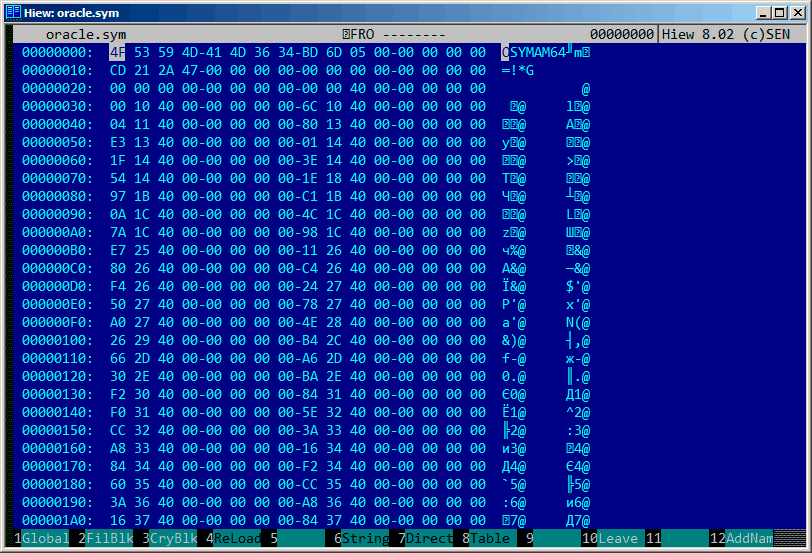
\includegraphics[scale=\FigScale]{ff/Oracle_SYM/whole64.png}
\caption{\RU{пример .SYM-файла из \oracle для win64}\EN{.SYM-file example from \oracle for win64}}
\label{fig:oracle_SYM_whole64}
\end{figure}

\RU{Так что да, все таблицы здесь имеют 64-битные элементы, даже смещения строк!}
\EN{So yes, all tables now has 64-bit elements, even string offsets!}
\RU{Сигнатура теперь}\EN{The signature is now} \TT{OSYMAM64}, \RU{чтобы отличить целевую платформу, 
я полагаю}\EN{to distinguish target platform, I suppose}.\\
\\
\RU{Вот и всё}\EN{This is it}!
\RU{Вот также моя библиотека в которой есть ф-ция для доступа к .SYM-файлам \oracle}\EN{Here is also my 
library in which I have function to access \oracle .SYM-files}:
\href{http://go.yurichev.com/17007}{GitHub}.
